\chapter{机械能及其守恒定律}

\section{功和功率}


1.功

(1)做功的两个要素

\ding{172}作用在物体上的\_\_力\_\_.

\ding{173}物体在力的方向上发生的\_\_位移\_\_.

(2)公式$W=Fl\cos \alpha$

\ding{172}$\alpha$是力与\_\_位移\_\_方向之间的夹角,l是物体对地的位移.

\ding{173}该公式只适用于\_\_恒力\_\_做功.

(3)功的正负

\ding{172}当$0\leq \alpha<\dfrac{\pi}{2}$时,$W>0$,力对物体做\_\_正功\_\_,是动力.

\ding{173}当$\dfrac{\pi}{2}<\alpha\leq π$时,$W<0$,力对物体做\_\_负功\_\_,或者说物体\_\_克服\_\_这个力做了功,是阻力.

\ding{174}当$\alpha=\dfrac{\pi}{2}$时,$W=0$,力对物体\_\_不做功\_\_.

2.功率

\begin{longtable}[]{@{}m{1.6cm}m{5cm}m{6cm}m{1cm}@{}}
\toprule
类别 & 定义 & 计算公式 & 单位\tabularnewline
\midrule
\endhead

平均功率&
力在一段时间内做功的平均快慢程度,大小等于功跟完成这些功所用时间的比值
& 
(1)$\bar{P}=\dfrac{W}{t}$

(2)$\bar{P}=F \bar{v}$,适用条件:F为恒力,且F与平均速度共线
&\multirow{4}{1cm}{瓦特(W)}
\tabularnewline
瞬时功率&
力在某一时刻做功的快慢程度
& \begin{minipage}[t]{0.4\columnwidth}\raggedright
(1)$P=Fv$,适用条件:F与瞬时速度v共线

(2)$t\rightarrow 0$,$P=\dfrac{W}{t}$为瞬时功率(不要求)\strut
\end{minipage} & \begin{minipage}[t]{0.22\columnwidth}\raggedright
\strut
\end{minipage}\tabularnewline

额定功率 & 
\begin{minipage}[t]{0.8\columnwidth}\raggedright
动力机械在正常条件下长时间工作的最大功率
\end{minipage} &
&\tabularnewline
实际功率 & 
\begin{minipage}[t]{0.8\columnwidth}\raggedright
动力机械工作时实际消耗的功率一般小于或等于额定功率
\end{minipage}
 &
&\tabularnewline
\bottomrule
\end{longtable}

\newpage
\subsection{恒力做功的计算}

1.恒力做的功

直接用$W=Fl\cos \alpha$计算.不论物体做直线运动还是曲线运动,上式均适用.

2.合外力做的功

法一:先求合外力$F_{\text{合}}$,再用$W_{\text{合}}=F_{\text{合}}l\cos \alpha$求功.适用于$F_{\text{合}}$为恒力的过程.

法二:先求各个力做的功$W_1$、$W_2$、$W_3$\ldots,再应用$W_{\text{合}}$=$W_1$+$W_2$+$W_3$+\ldots 求合外力做的功.

{[}例1{]}一物体静止在粗糙水平地面上.现用一大小为$F_1$的水平拉力拉动物体,经过一段时间后其速度变为v.若将水平拉力的大小改为$F_2$,物体从静止开始经过同样的时间后速度变为2v.对于上述两个过程,用$W_{f1}$、$W_{f2}$分别表示拉力$F_1$、$F_2$所做的功,$W_{f1}$、$W_{f2}$分别表示前后两次克服摩擦力所做的功,则( C )

A.$W_{f2}$\textgreater4$W_{f1}$,$W_{f2}$\textgreater2$W_{f1}$
B.$W_{f2}$\textgreater4$W_{f1}$,$W_{f2}$=2$W_{f1}$

C.$W_{f2}$\textless4$W_{f1}$,$W_{f2}$=2$W_{f1}$ D.$W_{f2}$\textless4$W_{f1}$,$W_{f2}$\textless2$W_{f1}$
\begin{solution}
	物体两次的加速度之比$a_{2}: a_{1}=\dfrac{2 v}{t}: \dfrac{v}{t}=2: 1$,位移之比$l_{2}: l_{1}=\dfrac{2 v}{2} t: \dfrac{v}{2} t=2: 1$,摩擦力之比$F_{\mathrm{f} 2}: F_{\mathrm{f} 1}=1: 1$,由牛顿第二定律得$F-F_f=ma$,则拉力之比$F_{2}: F_{1}=\left(m a_{2}+F_{\mathrm{f}}\right):\left(m a_{1}+F_{\mathrm{f}}\right)<2$,拉力做功之比$W_{f2}$:$W_{f1}$=$F_2$$l_2$:$F_1$$l_1$\textless4,克服摩擦力做功之比$W_{f2}:W_{f1}=\left(-F_{\mathrm{f} 2} l_{2}\right):\left(-F_{\mathrm{f} 1} l_{1}\right)=2: 1$,故选项C正确.
\end{solution}


\begin{center}
\includegraphics[width=0.70833in,height=0.125in]{media/image34.png}

\textbf{计算功时应注意的两个问题}
\end{center}


(1)计算恒力功的公式$W=Fl\cos \alpha$中位移``l''的意义

\ding{172}``l''应取作用点的位移;

\ding{173}``l''的取值一般以大地为参考系.

(2)力的独立性原理

求某个力做的功仅与该力及物体沿该力方向的位移有关,而与其他力是否存在、是否做功无关.
\subsection{功率的计算}

1.公式$P=\dfrac{W}{t}$ 和 $P=F v$的区别

$P=\dfrac{W}{t}$是功率的定义式,$P=F v$是功率的计算式.

2.平均功率的计算方法

(1)利用$\bar{P}=\dfrac{W}{t}$.

(2)利用$\bar{P}=F \bar{v} \cos \alpha,$ 其中 $\bar{v}$为物体运动的平均速度.

3.瞬时功率的计算方法

(1)利用公式$P=Fv\cos \alpha$,其中v为t时刻的瞬时速度.

(2)$P=F v_{F}$,其中vF为物体的速度v在力F方向上的分速度.

(3)$P=F_v v$,其中Fv为物体受到的外力F在速度v方向上的分力.

\begin{center}
\includegraphics[width=0.70833in,height=0.125in]{media/image34.png}

\textbf{求功率时应注意的问题}
\end{center}


(1)首先要明确所求功率是平均功率还是瞬时功率,对应于某一过程的功率为平均功率,对应于某一时刻的功率为瞬时功率.

(2)求功率大小时要注意F与v方向间的夹角$\alpha$对结果的影响.

(3)用$P=F \cdot \bar{v} \cos \alpha$求平均功率时,$\bar v$应容易求得,如求匀变速直线运动中某力的平均功率.

\subsection{机车启动问题}

1.两种启动方式的比较

\begin{longtable}[]{@{}m{1cm}m{1.5cm}m{5.5cm}m{5.3cm}@{}}
\toprule
\multicolumn{2}{c}{两种方式}
 & 以恒定功率启动 & 以恒定加速度启动 \tabularnewline
\midrule
\endhead
\multicolumn{2}{c}{P-t图和v-t图}
 &
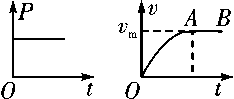
\includegraphics[width=1.0625in,height=0.44792in]{media/image210.png} &
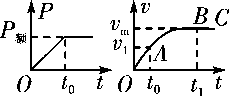
\includegraphics[width=1.04167in,height=0.4375in]{media/image211.png}\tabularnewline
\multirow{2}{1cm}{OA段}
&
过程分析 
&
$v \uparrow \Rightarrow F=\dfrac{P(\text { 不变 })}{v} \downarrow \Rightarrow a=\dfrac{F-F_{\text {阻 }}}{m}\downarrow$
&
$a=\dfrac{F-F_{\text {阻 }}}{m}$不变$ \Rightarrow F \text { 不变 } \boldsymbol{v} \uparrow \Rightarrow P=F v \uparrow$ 直到 $P_{\text {额}}=F v_{1}$\tabularnewline
 & 运动性质 & 加速度减小的加速直线运动 &
匀加速直线运动,维持时间$t_{0}=\dfrac{v_{1}}{a}$\tabularnewline
\multirow{2}{1cm}{AB段 }
& 过程分析 & $F=F_{\text {阻}} \Rightarrow a=0 \Rightarrow F$ 阻 $=\dfrac{P}{v_{\mathrm{m}}}$ & $v \uparrow \Rightarrow F=\dfrac{P_{\text {额 }}}{v} \downarrow \Rightarrow a=\dfrac{F-F_{\text {阻 }}}{m}$\tabularnewline
& 运动性质 & 以$v_m$匀速直线运动 & 加速度减小的加速运动\tabularnewline
\multicolumn{2}{c}{BC段} & 无 & $F=F_{\text {阻 }} \Rightarrow a=0 \Rightarrow$ 以 $v_{\mathrm{m}}=\dfrac{P_{\text {额}}}{F_{\text {阻 }}}$匀速运动\tabularnewline
\bottomrule
\end{longtable}

2.三个重要关系式

(1)无论哪种启动过程,机车的最大速度都等于其匀速运动时的速度,即$v_{\mathrm{m}}=\dfrac{P}{F_{\min }}=\dfrac{P}{F_{\text {阻 }}}$.(式中$F_{min}$为最小牵引力,其值等于阻力$F_{\text{阻}}$)

(2)机车以恒定加速度启动的运动过程中,匀加速过程结束时,功率最大,速度不是最大,即$v=\dfrac{P}{F}<v_{\mathrm{m}}=\dfrac{P}{F_{\text {阻 }}}$.

(3)机车以恒定功率运行时,牵引力做的功$W=Pt$.由动能定理$P t-F_{\text {阻 }}x=\Delta E_{\mathrm{k}}$.此式经常用于求解机车以恒定功率启动过程的位移大小.

{[}例3{]}在检测某种汽车性能的实验中,质量为$3\times 10^3kg$的汽车由静止开始沿平直公路行驶,达到的最大速度为40m/s,利用传感器测得此过程中不同时刻该汽车的牵引力F与对应速度v,并描绘出如图所示的$F-\dfrac{1}{v}$图象(图线ABC为汽车由静止到达到最大速度的全过程,AB、BO均为直线).假设该汽车行驶中所受的阻力恒定,根据图线ABC求:

(1)该汽车的额定功率;

(2)该汽车由静止开始运动,经过35 s达到最大速度40 m/s,其在BC段的位移.

\begin{center}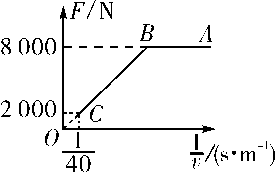
\includegraphics[width=1.25in,height=0.78125in]{media/image212.png}\end{center}

\begin{solution}
	(1)$8\times 10^4 W$ (2)75 m
\end{solution}
\begin{center}
\includegraphics[width=0.70833in,height=0.125in]{media/image34.png}

\textbf{分析机车启动时的注意事项}
\end{center}


(1)在用公式$P=Fv$计算机车的功率时,F是指机车的牵引力而不是机车所受到的合力.

(2)恒定功率下的加速过程一定不是匀加速运动,这种加速过程发动机做的功可用$W=Pt$计算,不能用$W=Fl$计算(因为F是变力).

(3)以恒定牵引力加速运动时的功率一定不恒定,这种加速运动过程发动机做的功常用$W=Fl$计算,不能用$W=Pt$计算(因为功率P是变化的).

\subsection{变力做功的求解方法}

1.平均力法

若物体受到的力的方向不变,而大小随位移是成线性变化的,即力均匀变化时,则可以认为物体受到一大小为$\bar{F}=\dfrac{F_{1}+F_{2}}{2}$的恒力作用,$F_1$、$F_2$分别为物体初、末态所受到的力,然后用公式$\bar{F}=\dfrac{F_{1}+F_{2}}{2}$求此力所做的功.



2.F-x图象法

在F-x图象中,图线与x轴所围``面积''的代数和就表示力F在这段位移上所做的功,且位于x轴上方的``面积''为正,位于x轴下方的``面积''为负,但此方法只适用于便于求图线所围面积的情况.

{[}例5{]}(2018·重庆模拟)轻质弹簧右端固定在墙上,左端与一质量m=0.5
kg的物块相连,如图甲所示,弹簧处于原长状态,物块静止且与水平面间的动摩擦因数$\mu$=0.2.以物块所在处为原点,水平向右为正方向建立x轴,现对物块施加水平向右的外力F,F随x轴坐标变化的情况如图乙所示,物块运动至x=0.4
m处时速度为零,则此时弹簧的弹性势能为(g=10 $m/s^2$)( A )

\begin{center}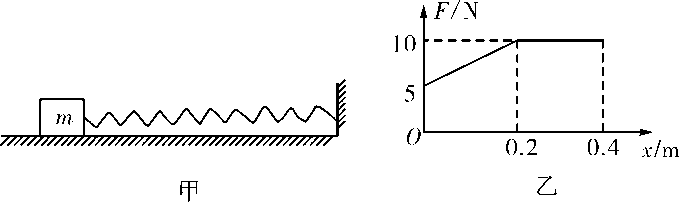
\includegraphics[width=3.08333in,height=0.91667in]{media/image213.png}\end{center}

A.3.1 J B.3.5 J

C.1.8 J D.2.0 J

3.等效转换法

若某一变力做的功和某一恒力做的功相等,即效果相同,则可以通过计算该恒力做的功,求出该变力做的功,从而使问题变得简单,也就是说通过关联点,将变力做功转化为恒力做功,这种方法称为等效转换法.


4.动能定理法

动能定理既适用于直线运动,也适用于曲线运动,既适用于求恒力做功也适用于求变力做功.因使用动能定理可由动能的变化来求功,所以动能定理是求变力做功的首选.



5.微元法

当物体在变力的作用下做曲线运动时,若力的方向与物体运动的切线方向之间的夹角不变,可将曲线分成无限个小元段,每一小元段可认为恒力做功,总功即为各个小元段做功的代数和.通过微元法不难得到,在往返的运动中,摩擦力、空气阻力做的功,其大小等于力和路程的乘积.


\begin{center}
\includegraphics[width=0.70833in,height=0.125in]{media/image13.png}

\textbf{变力做功的求解方法}
\end{center}


(1)平均力法:力的方向恒定,大小随位移线性变化,可用平均力法求变力做的功.

(2)F-x图象法:已知F-x图象,可以根据``面积''求变力做的功.

(3)等效转换法:变力功与恒力功相等,即等效,可以用``化变为恒''的等效转换法求变力做的功.

(4)动能定理法:无论直线运动还是曲线运动,只要知道了初末状态动能的变化,就可以用动能定理法求变力做的功.

(5)变力作用下的曲线运动过程,其元过程可以看成恒力作用过程,可以用微元法求变力做的功.

\newpage
\section{动能定理及其应用}


1.动能

(1)定义:物体由于\_\_运动\_\_而具有的能.

(2)公式:$E_{\mathrm{k}}=\dfrac{1}{2} m v^{2}$.

(3)单位:\_\_焦耳\_\_,$1 J=1 N\cdot m=1 kg\cdot m^2/s^2$.

(4)标矢性:动能是\_\_标量\_\_,只有正值,动能与速度方向\_\_无关\_\_.

(5)动能的变化:物体\_\_末动能\_\_与\_\_初动能\_\_之差,即$\Delta E_k=\dfrac{1}{2}mv_2^{2}-\dfrac{1}{2}mv_1^{2}$.

2.动能定理

(1)内容:在一个过程中合力对物体所做的功,等于物体在这个过程中\_\_动能的变化\_\_.

(2)表达式:$W=\Delta E_k=E_{k2}-E_{k1}=\dfrac{1}{2}mv_2^{2}-\dfrac{1}{2}mv_1^{2}$.

(3)物理意义:\_\_合力\_\_的功是物体动能变化的量度.

(4)适用条件

\ding{172}动能定理既适用于直线运动,也适用于\_\_曲线运动\_\_.

\ding{173}既适用于恒力做功,也适用于\_\_变力\_\_做功.

\ding{174}力可以是各种性质的力,既可以同时作用,也可以\_\_分阶段\_\_作用.

\newpage
\subsection{对动能定理的理解}

1.对``外力''的两点理解

(1)``外力''指的是合力,重力、弹力、摩擦力、电场力、磁场力或其他力,他们可以同时作用,也可以不同时作用.

(2)既可以是恒力,也可以是变力.

2.``=''体现的两个关系

\begin{center}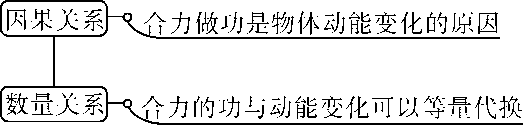
\includegraphics[width=2.37708in,height=0.56597in]{media/image223.png}\end{center}

{[}例1{]}(2018·湖北宜昌模拟)一辆汽车在平直公路上行驶,在汽车的速度从0增大到v的过程中,发动机做的功为$W_1$;在汽车的速度从v增大到2v的过程中,发动机做的功为$W_2$.设汽车在行驶过程中所受阻力和发动机的牵引力都不变,则有( B )

A.$W_2=2W_1$ B.$W_2=3W_1$

C.$W_2=4W_1$ D.$W_2=W_1$

\begin{solution}
	设汽车发动机的牵引力为F,汽车所受的阻力为$F_f$,两个过程中汽车的位移分别为$l_1$、$l_2$,则由动能定理得$(F-F_f)l_1=\dfrac{1}{2} m v^{2}-0,\left(F-F_{\mathrm{f}}\right) l_{2}=\dfrac{1}{2} m(2 v)^{2}-\dfrac{1}{2} m v^{2},$ 解得 $l_{2}=3 l_{1}, \quad$ 又 $W_{1}=F l_{1}, \quad W_{2}=F l_{2}, \quad$ 可得 $W_{2}=3 W_{1}$,选项B正确.
\end{solution}
\begin{center}
\includegraphics[width=0.70764in,height=0.12292in]{media/image13.png}

\textbf{应用动能定理解题应抓好``两状态一过程''}
\end{center}


``两状态'',即明确研究对象的始、末状态的速度或动能情况;``一过程'',即明确研究过程,确定这一过程研究对象的受力情况和位置变化或位移信息.高中阶段动能定理中的位移和速度应以地面或相对地面静止的物体为参考系.


\subsection{动能定理的应用}

{[}例2{]}(2018·河南郑州模拟)2014年全国多地雾霾频发,且有愈演愈烈的趋势,空气质量问题备受关注.在雾霾天气下,能见度下降,机动车行驶速度降低,道路通行效率下降,对城市快速路、桥梁和高速公路的影响很大,已知汽车保持匀速正常行驶时受到的阻力为$F_{f1}=0.2mg$,刹车时受到的阻力为$F_{f2}=0.5mg$,重力加速度为$g=10m/s^2$.

(1)若汽车在雾霾天行驶的速度为$v_1=36km/h$,则刹车后经过多长时间才会停下来?

(2)若前车因故障停在车道上,当质量为m=1 200kg的后车距离已经停止的前车为x=22.5m处紧急刹车,刚好不与前车相撞,则后车正常行驶时的功率为多大?
\begin{solution}
	(1)2 s (2)$3.6\times 10^4 W$
\end{solution}


\begin{center}
\includegraphics[width=0.70764in,height=0.12292in]{media/image25.png}

\textbf{应用动能定理解题步骤}
\end{center}


\begin{center}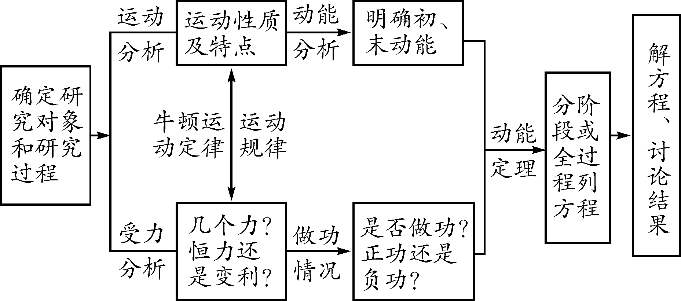
\includegraphics[width=3.09444in,height=1.36806in]{media/image224.png}\end{center}

\subsection{动能定理与图象结合问题}

解决物理图象问题的基本步骤

(1)观察题目给出的图象,弄清纵坐标、横坐标所对应的物理量及图线所表示的物理意义.

(2)根据物理规律推导出纵坐标与横坐标所对应的物理量间的函数关系式.

(3)将推导出的物理规律与数学上与之相对应的标准函数关系式相对比,找出图线的斜率、截距、图线的交点,以及图线下的面积所对应的物理意义,分析解答问题.或者利用函数图线上的特定值代入函数关系式求物理量.

{[}例3{]}(2017·湖北黄石调研)用传感器研究质量为2
kg的物体由静止开始做直线运动的规律时,在计算机上得到0~6
s内物体的加速度随时间变化的关系如图所示.下列说法正确的是( D )

\begin{center}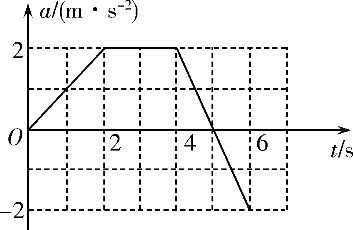
\includegraphics[width=1.60347in,height=1.04722in]{media/image225.png}\end{center}

A.0~6 s内物体先向正方向运动,后向负方向运动

B.0~6 s内物体在4 s时的速度最大

C.物体在2~4 s内速度不变

D.0~4 s内合力对物体做的功等于0~6 s内合力做的功

\begin{center}
\includegraphics[width=0.70764in,height=0.12292in]{media/image13.png}

\textbf{图象所围``面积''的意义}
\end{center}


(1)v-t图:由公式x=vt可知,v-t图线与坐标轴围成的面积表示物体的位移.

(2)a-t图:由公式$\Delta$v=at可知,a-t图线与坐标轴围成的面积表示物体速度的变化量.

(3)F-x图:由公式W=Fx可知,F-x图线与坐标轴围成的面积表示力所做的功.

(4)P-t图:由公式W=Pt可知,P-t图线与坐标轴围成的面积表示力所做的功.


\subsection{动能定理与圆周运动结合}

1.圆周运动属于曲线运动,若只涉及位移和速度而不涉及时间,应优先考虑用动能定理列式求解.

2.用动能定理解题,关键是对研究对象进行准确的受力分析及运动过程分析,并画出物体运动过程的草图,让草图帮助我们理解物理过程和各量关系.

{[}例4{]}(2018·湖北武汉模拟)如图所示,半径$r_{1}=\dfrac{2}{5} \sqrt{2} \mathrm{m}$的圆弧轨道AB与水平轨道BC相切于B点,CD为$r_2=0.40m$的半圆轨道,另一半径R=1.00
m的圆弧轨道EF与CD靠近,E点略低于D点.一质量m=1
kg的小物块(可视为质点)从A点以初速度$v_0=2m/s$沿轨道下滑,在AB段运动过程中始终受到竖直向上的F=10
N的力作用,进入BC段后撤去.已知AB高度为h,BC长L=1.00
m,小物块与BC间动摩擦因数$\mu$=0.2,其余光滑,EF轨道对应的圆心角$\theta=60^\circ$,所有轨道均固定在同一竖直平面内,不考虑小物块在各轨道相接处的能量损失,忽略空气阻力,g取$10m/s^2$.求:

(1)当小物块沿圆弧轨道AB运动到B点时,轨道对小物块的作用力大小;

(2)若小物块在B点的速度为5
m/s,且在刚进入BC段时撤去力F,请通过计算判断小物块能否通过D点;

(3)小物块能进入EF轨道,且不越过F点,小物块在D点的速度范围.

\begin{center}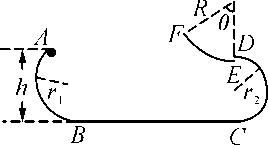
\includegraphics[width=1.21667in,height=0.66042in]{media/image226.png}\end{center}

\begin{solution}
	(1)$5 \sqrt{2} \mathrm{N}$ (2)见解析 (3)$2 m/s\leq v_D\leq  m/s$.
\end{solution}
\begin{center}
\includegraphics[width=0.70764in,height=0.12292in]{media/image13.png}

\textbf{动能定理在圆周运动中的应用}
\end{center}


竖直面内圆周运动经常考查最高点和最低点,最高点的速度和最低点的速度可以通过动能定理联系起来,所以竖直面内的圆周运动经常和动能定理结合考查.


\subsection{用动能定理解决多过程问题}

1.运用动能定理解决问题时,选择合适的研究过程能使问题得以简化.当物体的运动过程包含几个运动性质不同的子过程时,可以选择一个、几个或全部子过程作为研究过程.

2.当选择全部子过程作为研究过程,涉及重力、大小恒定的阻力或摩擦力做功时,要注意运用它们的做功特点:

(1)重力的功取决于物体的初、末位置,与路径无关.

(2)大小恒定的阻力或摩擦力做的功等于力的大小与路程的乘积.

{[}例5{]}(2018·湖南联考)如图所示,光滑的水平轨道MN右端N处与水平传送带理想连接,传送带水平长度L=1.6
m,皮带以恒定速率v逆时针匀速运动,传送带的右端平滑连接着一个固定在竖直平面内、半径为R=0.4
m的光滑半圆轨道PQ;质量为m=0.2
kg且可视为质点的滑块A置于水平导轨MN上,开始时滑块A与墙壁之间有一压缩的轻弹簧,系统处于静止状态,现松开滑块A,弹簧伸长,滑块脱离弹簧后滑上传送带,从右端滑出并沿半圆轨道运动到最高点Q后水平飞出,又正好落回N点.已知滑块A与传送带之间的动摩擦因数$\mu=0.25$,取$g=10m/s^2$.求:

\begin{center}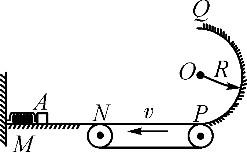
\includegraphics[width=1.12292in,height=0.68889in]{media/image227.png}\end{center}

(1)滑块A在半圆轨道P处对轨道的压力;

(2)压缩的轻弹簧的弹性势能$E_p$.
\begin{solution}
	(1)18 N (2)4 J
\end{solution}

\newpage
\section{机械能守恒定律及其应用}


1.重力做功与重力势能的关系

(1)重力做功的特点

\ding{172}重力做功与\_\_路径\_\_无关,只与始末位置的\_\_高度差\_\_有关.

\ding{173}重力做功不引起物体\_\_机械能\_\_的变化.

(2)重力势能

\ding{172}表达式:$E_p=mgh$.

\ding{173}重力势能的特点

重力势能是物体和\_\_地球\_\_所共有的,重力势能的大小与参考平面的选取\_\_有关\_\_,但重力势能的变化与参考平面的选取\_\_无关\_\_.

(3)重力做功与重力势能变化的关系

\ding{172}定性关系:重力对物体做正功,重力势能\_\_减小\_\_;重力对物体做负功,重力势能\_\_增大\_\_;

\ding{173}定量关系:重力对物体做的功等于物体重力势能增量的负值.即$W_G=-(E_{p2}-E_{p1})=-\Delta E_p$.

2.弹性势能

(1)定义:发生\_\_弹性形变\_\_的物体之间,由于有弹力的相互作用而具有的势能.

(2)弹力做功与弹性势能变化的关系:弹力做正功,弹性势能\_\_减小\_\_;弹力做负功,弹性势能\_\_增加\_\_.即$W=-\Delta E_p$.

3.机械能守恒定律及其应用

(1)内容

在只有\_\_重力\_\_或\_\_弹簧弹力\_\_做功的物体系统内,动能与势能可以相互转化,而总的机械能\_\_保持不变\_\_.

(2)守恒条件

只有\_\_重力或弹簧弹力\_\_做功.


\newpage
\subsection{机械能守恒的判断方法}

1.机械能守恒的条件:只有重力或系统内的弹力做功.

2.机械能守恒的判断方法:

(1)从机械能的定义直接判断:若物体动能、势能均不变,机械能不变.若一个物体动能不变,重力势能变化,或重力势能不变,动能变化或动能和重力势能同时增加(或减小),其机械能一定变化.

(2)用做功判断:若物体或系统只有重力(或弹簧的弹力)做功,虽受其他外力,但其他外力不做功,则机械能守恒.

(3)用能量转化来判断:若物体系统中只有动能和势能的相互转化而无机械能与其他形式的能的转化,则物体系统的机械能守恒.

{[}例1{]}(2018·广西南宁调研)在如图所示的物理过程示意图中,甲图为一端固定有小球的轻杆,从右偏上$30^\circ$角释放后绕光滑支点摆动;乙图为末端固定有A、B两小球的轻质直角架,释放后绕通过直角顶点的固定轴O无摩擦转动;丙图为置于光滑水平面上的A、B两小车,B静止,A获得一向右的初速度后向右运动,某时刻连接两车的细绳绷紧,然后带动B车运动;丁图为置于光滑水平面上的带有竖直支架的小车,把用细绳悬挂的小球从图示位置释放,小球开始摆动.则关于这几个物理过程(空气阻力忽略不计),下列判断中正确的是( A )

\begin{center}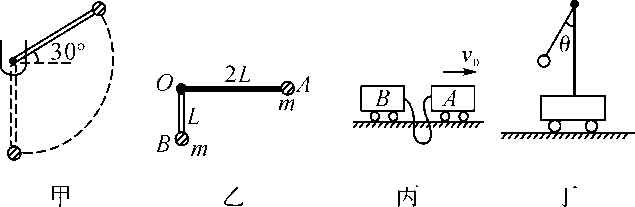
\includegraphics[width=2.88681in,height=0.94306in]{media/image232.png}\end{center}

A.甲图中小球机械能守恒

B.乙图中小球A的机械能守恒

C.丙图中两车组成的系统机械能守恒

D.丁图中小球的机械能守恒

\begin{center}
\includegraphics[width=0.70764in,height=0.12292in]{media/image44.png}\end{center}

(1)机械能守恒的条件绝不是合外力的功等于零,更不是合外力为零;``只有重力做功''不等于``只受重力作用''.

(2)分析机械能是否守恒时,必须明确要研究的系统.


\subsection{单个物体机械能守恒定律的应用}

\begin{center}
\includegraphics[width=0.70764in,height=0.12292in]{media/image37.png}

\textbf{机械能守恒定律的应用技巧}
\end{center}


(1)机械能守恒定律是一种``能---能转化''关系,其守恒是有条件的.因此,应用时首先要对研究对象在所研究的过程中机械能是否守恒做出判断.

(2)如果系统(除地球外)只有一个物体,用守恒观点列方程较方便;对于由两个或两个以上物体组成的系统,用转化或转移的观点列方程较简便.



\newpage
\subsection{多个物体的机械能守恒}

1.对多个物体组成的系统,要注意判断物体运动过程中系统的机械能是否守恒.

判断方法:看是否有其他形式的能与机械能相互转化.

2.三种守恒表达式的比较

\begin{longtable}[]{@{}m{0.8cm}m{3.5cm}m{5cm}m{4cm}@{}}
\toprule
角度 & 公式 & 意义 & 注意事项\tabularnewline
\midrule
\endhead

守恒
观点
&
$E_{k1}+E_{p1}=E_{k2}+E_{p2}$
&
系统的初状态机械能的总和与末状态机械能的总和相等
&
初、末状态必须用同一零势能面计算势能
\tabularnewline

转化
观点
&
$\Delta E_k=-\Delta E_p$
&
系统减少(或增加)的重力势能等于系统增加(或减少)的动能
&
应用时关键在于分清重力势能的增加量和减少量,可不选零势能面而直接计算初、末状态的势能差
\tabularnewline

转移
观点
&
$\Delta E_{A\text{增}}=
\Delta E_{B\text{减}}$
&
若系统由A、B两物体组成,则A物体机械能的增加量与B物体机械能的减少量相等
&
常用于解决两个或多个物体组成的系统的机械能守恒问题\tabularnewline
\bottomrule
\end{longtable}

\begin{center}
\includegraphics[width=0.70764in,height=0.12292in]{media/image13.png}

\textbf{多物体机械能守恒问题}
\end{center}


(1)多物体机械能守恒问题的分析方法

\ding{172}对多个物体组成的系统要注意判断物体运动过程中,系统的机械能是否守恒;

\ding{173}注意寻找用绳或杆相连接的物体间的速度关系和位移关系;

\ding{174}列机械能守恒方程时,一般选用$\Delta E_k=-\Delta E_p$的形式.

(2)多物体机械能守恒问题的三点注意

\ding{172}正确选取研究对象;

\ding{173}合理选取物理过程;

\ding{174}正确选取机械能守恒定律常用的表达形式列式求解.


\subsection{绳索、链条类机械能守恒问题}

对绳索、链条之类的问题,由于在考查过程中其常发生形变,其重心位置对物体来说并不是固定不变的,能否正确确定重心的位置,是解决该类问题的关键.一般情况下常分段考虑各部分的势能,并用各部分势能之和作为系统总的重力势能,至于参考平面,可任意选取,但以系统初、末状态重力势能便于表示为宜.



\newpage
\section{功能关系 能量守恒定律} 


1.功能关系

(1)功是\_\_能量转化\_\_的量度,即做了多少功就有\_\_多少能量\_\_发生了转化.

(2)做功的过程一定伴随着\_\_能量的转化\_\_,\_\_能量的转化\_\_可以通过做功来实现.

2.能量守恒定律

(1)能量守恒定律的内容:能量既不会凭空\_\_产生\_\_,也不会凭空消失,它只能从一种形式\_\_转化\_\_为另一种形式,或者从一个物体\_\_转移\_\_到别的物体,在转化或转移的过程中,能量的总量\_\_保持不变\_\_.

(2)能量守恒定律的表达式:$\Delta E_{\text{减}}=$\_\_$\Delta E_{\text{增}}$\_\_.

(3)对定律的理解

\ding{172}某种形式的能减少,一定存在其他形式的能增加,且减少量和增加量一定相等.

\ding{173}某个物体的能量减少,一定存在其他物体的能量增加,且减少量和增加量一定相等.

这也是我们列能量守恒定律方程式的两条基本思路.

\newpage
\subsection{对功能关系的理解}

1.对功能关系的理解

(1)做功的过程就是能量转化的过程.不同形式的能量发生相互转化可以通过做功来实现.

(2)功是能量转化的量度.功和能的关系,一是体现在不同性质的力做功,对应不同形式的能转化,具有一一对应关系,二是做功的多少与能量转化的多少在数值上相等.

2.几种常见的功能关系及其表达式

\begin{longtable}[]{@{}m{2cm}m{1.5cm}m{10cm}@{}}
\toprule
各种力做功 & 对应能的变化 & 定量的关系\tabularnewline
\midrule
\endhead
合力的功 & 动能变化 &
合力对物体做功等于物体动能的增量$W_{\text{合}}=E_{k2}-E_{k1}$\tabularnewline
重力的功 & 重力势能变化 &
重力做正功,重力势能减少,重力做负功,重力势能增加,且$W_G=-\Delta E_p=E_{p1}-E_{p2}$\tabularnewline
弹簧弹力的功 & 弹性势能变化 &
弹力做正功,弹性势能减少,弹力做负功,弹性势能增加,且$W_{\text{弹}}=-\Delta E_p=E_{p1}-E_{p2}$\tabularnewline
只有重力、弹簧弹力的功 & 不引起机械能变化 &
机械能守恒$\Delta E=0$\tabularnewline
非重力和弹力的功 & 机械能变化 &
除重力和弹力之外的其他力做正功,物体的机械能增加,做负功,机械能减少,且$W_{\text{其他}}\neq E$\tabularnewline
电场力的功 & 电势能变化 &
电场力做正功,电势能减少,电场力做负功,电势能增加,且$W_{\text{电}}=-\Delta$Ep\tabularnewline
滑动摩擦力的功 & 内能变化 &
滑动摩擦力做功引起系统内能增加$\Delta E_{\text{内}}=F_fl_{\text{相对}}$\tabularnewline
\bottomrule
\end{longtable}

{[}例1{]}(2017·全国卷\uppercase\expandafter{\romannumeral3})如图,一质量为m、长度为l的均匀柔软细绳PQ竖直悬挂.用外力将绳的下端Q缓慢地竖直向上拉起至M点,M点与绳的上端P相距l.重力加速度大小为g.在此过程中,外力做的功为( A )

\begin{center}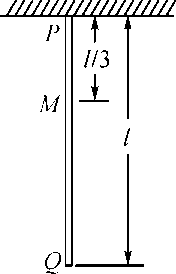
\includegraphics[width=0.80208in,height=1.24514in]{media/image240.png}\end{center}

A.mgl   B.mgl

C.mgl   D.mgl

\begin{center}
\includegraphics[width=0.70764in,height=0.12292in]{media/image13.png}

\textbf{功能关系的选用原则}
\end{center}


(1)在应用功能关系解决具体问题的过程中,若只涉及动能的变化用动能定理分析.

(2)只涉及重力势能的变化用重力做功与重力势能变化的关系分析.

(3)只涉及机械能的变化用除重力和弹力之外的力做功与机械能变化的关系分析.

(4)只涉及电势能的变化用电场力做功与电势能变化的关系分析.


\subsection{摩擦力做功与能量转化}

1.静摩擦力做功

(1)静摩擦力可以做正功,也可以做负功,还可以不做功.

(2)相互作用的一对静摩擦力做功的代数和总等于零.

(3)静摩擦力做功时,只有机械能的相互转移,不会转化为内能.

2.滑动摩擦力做功的特点

(1)滑动摩擦力可以做正功,也可以做负功,还可以不做功.

(2)相互间存在滑动摩擦力的系统内,一对滑动摩擦力做功将产生两种可能效果:

\ding{172}机械能全部转化为内能;

\ding{173}有一部分机械能在相互摩擦的物体间转移,另外一部分转化为内能.

(3)摩擦生热的计算:$Q=F_fx_{\text{相对}}$.其中$x_{\text{相对}}$为相互摩擦的两个物体间的相对路程.

从功的角度看,一对滑动摩擦力对系统做的功等于系统内能的增加量;从能量的角度看,其他形式能量的减少量等于系统内能的增加量.

{[}例2{]}(2018·河北保定调研)(多选)如图所示,足够长的传送带与水平方向的夹角为$\theta$,物块a通过平行于传送带的轻绳跨过光滑定滑轮与物块b相连,b的质量为m,开始时,a、b及传送带均静止且a不受传送带摩擦力作用,现让传送带逆时针匀速转动,则在b上升h高度(未与滑轮相碰)过程中( BC )

\begin{center}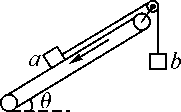
\includegraphics[width=0.82083in,height=0.50972in]{media/image241.png}\end{center}

A.物块a的重力势能减少了$mgh\sin \theta$

B.摩擦力对a做的功大于a的机械能的增加量

C.摩擦力对a做的功等于物块a、b动能增加量之和

D.任意时刻,重力对a、b做功的瞬时功率大小不相等
\begin{solution}
	开始时,a、b及传送带均静止且a不受传送带摩擦力作用,有$m_ag\sin\theta=m_bg$,则$m_{a}=\dfrac{m_{b}}{\sin \theta}=\dfrac{m}{\sin \theta}$,b上升h,则a下降$h\sin\theta$,则a重力势能的减少量为$\Delta E_{pa}=m_agh\sin\theta=mgh$,故选项A错误;根据能量守恒得系统机械能增加,摩擦力对a做的功等于a、b机械能的增加量,所以摩擦力对a做的功大于a机械能的增加量;由A分析可知系统重力势能不变,所以摩擦力做的功等于系统动能的增加量,故选项B、C正确;任意时刻,a、b的速率相等,对b,重力的瞬时功率大小$P_b=mgv$,对a有$P_a=m_agv\sin\theta=mgv$,所以重力对a、b做功的瞬时功率大小相等,故选项D错误.
\end{solution}


\begin{center}
\includegraphics[width=0.70764in,height=0.12292in]{media/image13.png}

\textbf{求解相对滑动过程中能量转化问题的思路}
\end{center}


(1)正确分析物体的运动过程,做好受力分析.

(2)利用运动学公式,结合牛顿第二定律分析物体的速度关系及位移关系.

(3)公式$Q=F_fx_{\text{相对}}$中x相对为两接触物体间的相对位移,若物体在传送带上做往返运动时,则x相对为总的相对路程.

\newpage
\subsection{能量转化规律的应用}

1.应用能量守恒定律的基本思路

(1)某种形式的能减少,一定存在其他形式的能增加,且减少量和增加量一定相等;

(2)某个物体的能量减少,一定存在其他物体的能量增加,且减少量和增加量一定相等.

2.应用能量守恒定律解题的步骤

(1)分清有多少形式的能(动能、势能、内能等)发生变化.

(2)明确哪种形式的能量增加,哪种形式的能量减少,并且列出减少的能量$\Delta E_{\text{减}}$和增加的能量$\Delta E_{\text{增}}$的表达式.

(3)列出能量守恒关系式$\Delta E_{\text{减}}\neq E_{\text{增}}$.

{[}例3{]}(2017·江苏启东一模)如图所示,一物体质量m=2
kg,在倾角$\theta$=$37^\circ$的斜面上的A点以初速度$v_0=3m/s$下滑,A点距弹簧上端B的距离AB=4
m.当物体到达B点后将弹簧压缩到C点,最大压缩量BC=0.2
m,然后物体又被弹簧弹上去,弹到的最高位置为D点,D点距A点的距离AD=3
m.挡板及弹簧质量不计,g取$10m/s^2$,$\sin 37^\circ=0.6$.求:

\begin{center}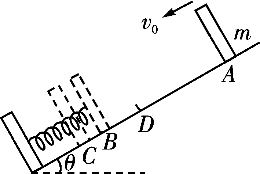
\includegraphics[width=1.17917in,height=0.79236in]{media/image242.png}\end{center}

(1)物体与斜面间的动摩擦因数$\mu$;

(2)弹簧的最大弹性势能Epm.
\begin{solution}
	(1)0.52 (2)24.5 J
\end{solution}


\begin{center}
\includegraphics[width=0.70764in,height=0.12292in]{media/image13.png}

\textbf{能量问题的解题方法}
\end{center}


(1)涉及能量转化问题的解题方法

\ding{172}当涉及滑动摩擦力做功,机械能不守恒时,一般应用能的转化和守恒定律.

\ding{173}解题时,首先确定初、末状态,然后分析状态变化过程中哪种形式的能量减少,哪种形式的能量增加,求出减少的能量总和$\Delta E_{\text{减}}$和增加的能量总和$\Delta E_{\text{增}}$,最后由$\Delta E_{\text{减}}\neq E_{\text{增}}$列式求解.

(2)涉及弹簧类能量问题的解题方法

两个或两个以上的物体与弹簧组成的系统相互作用的过程,具有以下特点:

\ding{172}能量变化上,如果只有重力和系统内弹簧弹力做功,系统机械能守恒.

\ding{173}如果系统中每个物体除弹簧弹力外所受合外力为零,则当弹簧伸长或压缩到最大程度时两物体速度相同.

\ding{174}当弹簧为自然状态时系统内某一端的物体具有最大速度.

